\chapter{Implementation}

The following chapter describes design and implementation of the PBTC control algorithm and software required for simulation. To produce a representative comparison with existing SCATS-based systems, creating a realistic simulation environment was a key implementation challenge, and a primary objective of this project. The outcomes discussed in this chapter are:

\begin{itemize}
\item using the open-source software package MovSim as a framework for implementation and simulation,
\item implementing a simulation scenario for development and evaluation,
\item design and implementation of a modular traffic control framework within the MovSim project, supporting development of the PBTC control algorithm and allowing for future control algorithms to be added easily,
\item implementation of the PBTC control algorithm within the simulation tool,
\item development of a parser for SCATS log files, to allow for traffic flow rates and traffic signal phase timings to be read from a SCATS log file and used in simulation,
\end{itemize}

\section{Simulator Implementation}

A primary challenge of measuring and evaluating performance of an adaptive traffic control system is the requirement to simulate realistic traffic conditions with sufficiently measurable results. Software for simulating traffic control methods is typically developed by vendors of a particular system and as such is proprietary and not available for research. Because of this, an open-source tool called Movsim has been used to develop and evaluate the PBTC system. 

Movsim (Multi-model Open-source Vehicular-traffic Simulator) is an open-source, Java-based traffic simulator implementing multiple time-continuous, car-following traffic models designed for investigating traffic dynamics; currently under active development. Movsim is based upon the work of \citeasnoun{kesting2013traffic} and implements a wide range of configurable vehicle-following, acceleration, and lane changing models that determine individual vehicle movement within the simulation.

\begin{figure}[]
\centering
	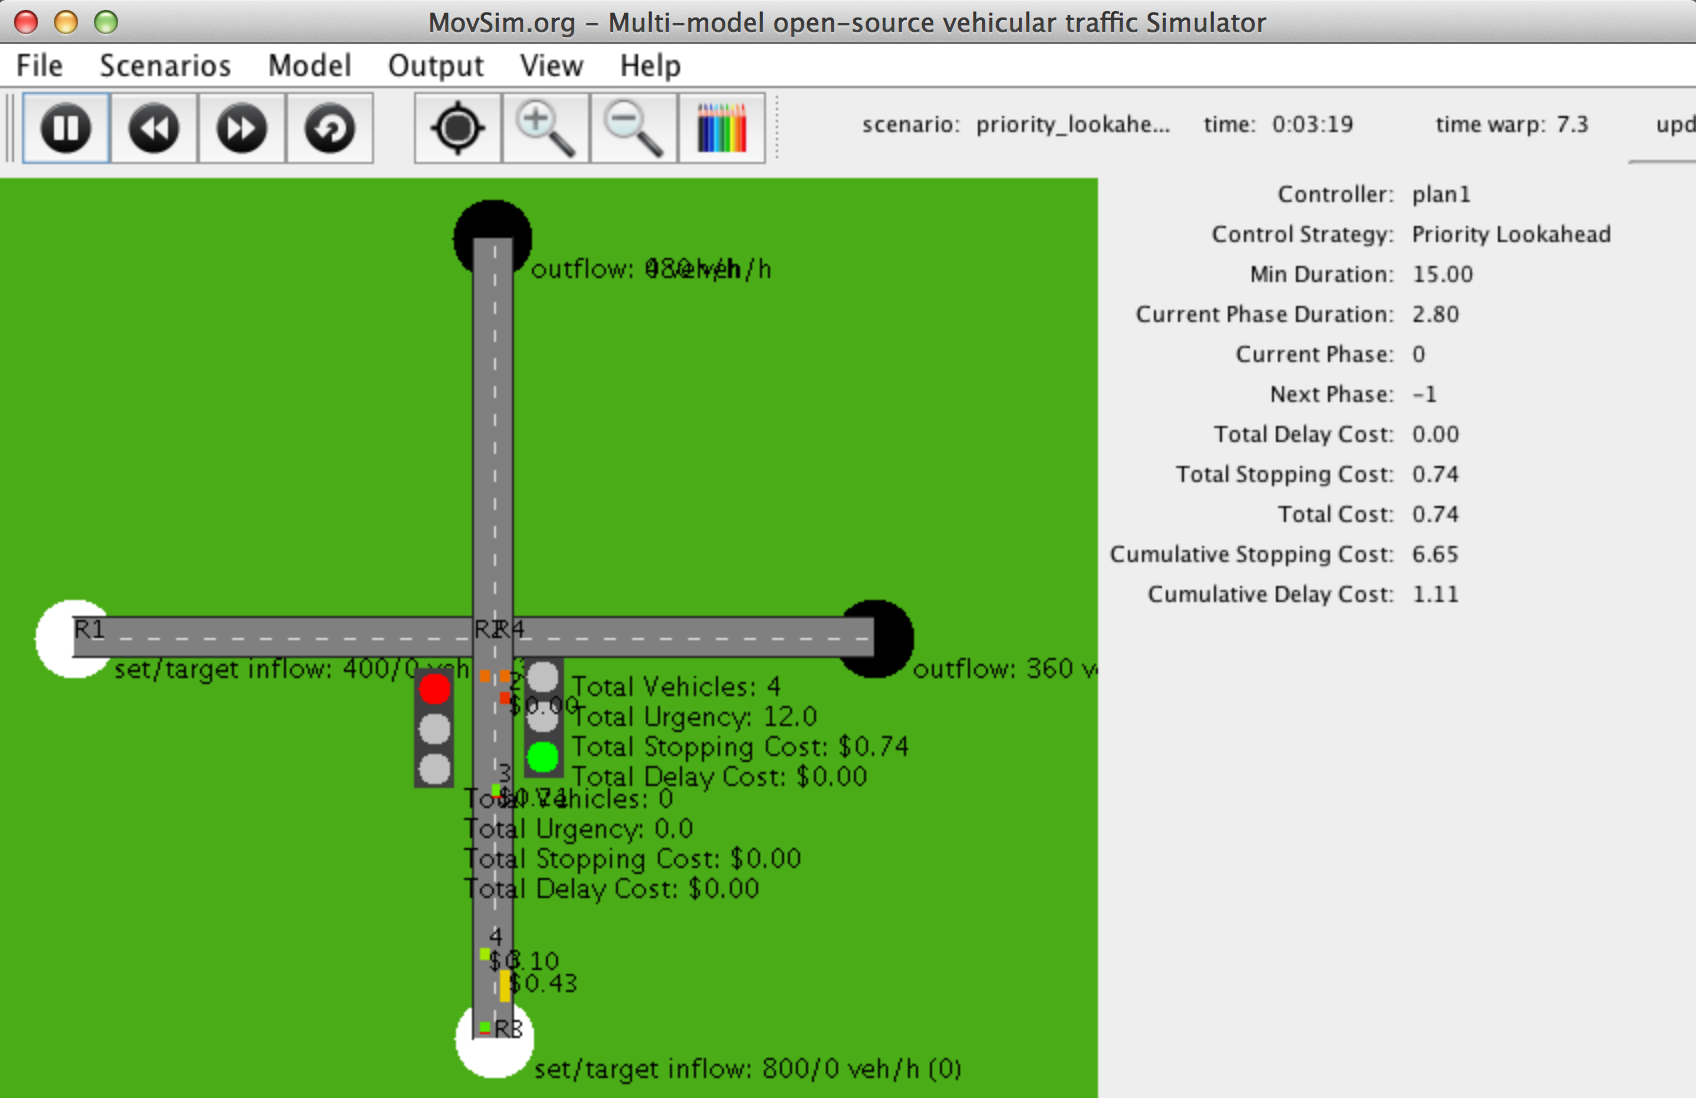
\includegraphics[scale=0.35]{movsim-interface.png}
	\caption{ A screenshot of the MovSim Graphical User Interface running a simulation of the four-way intersection scenario used during design and evaluation of the PBTC control system. }
\label{intersectiondiagram}
\end{figure}

% MovSim also has a stand-alone visualisation engine that is used to view the progress of a simulation at runtime. Visualising the state of running simulations is beneficial for validating intersection layouts and exploring the interaction between individual vehicles and traffic signals.

All software artefacts produced during this project were implemented within a fork of the Movsim project. Using Git as a source code management tool allowed for general purpose features and improvements to be committed back to the original Movsim repository, and specific changes required by this project to be maintained within a local project.

Limitations of using the MovSim project as a base simulation tool for the PBTC system include lack of support for bi-directional traffic flow and turning behaviour at intersections, both requirements for accurate modeling of a real world road network. Both of these features are areas of future development for the MovSim project. The sophisticated traffic modeling capabilities of the MovSim application, have outweighed these limitations during development of the PBTC system.

%\item \textbf{Fuel consumption models}, MovSim includes a fuel consumption package that can retrospectively analyse individual or collective consumption for a simulation. Fuel consumption models can be applied to calculate instantaneous fuel costs and the cost of stopping, related to the priority of a vehicle. 

\section{Scenario Design}

The MovSim simulator is designed to be highly configurable and uses XML files as specifications for the simulations that will be executed. One of the two road network description files required by MovSim is an OpenDrive network specification file which defines the geometry, order, and connections between roads which are structured in XML. OpenDrive is an "open file format for the logical description of road networks" \cite{opendrive}. The format is extremely descriptive and supports a large number of geometric constructs to generate realistic road networks. As MovSim required the use of OpenDrive, no alternative road network description formats are discussed here.

The intersection configuration designed and implemented for evaluation purposes within this project consists of two one-way approaches, each with two vehicle lanes and was based on availability of data for real-world intersections in Wellington City. As a four-way intersection configuration is a common design, the configuration files were submitted back to the Movsim repository as an example, and accepted by the Movsim authors. 

% include snippet example in appendix?

Although OpenDrive supports a large number of realistic road network configurations, the implementation supported within the MovSim simulator is limited to a subset of these. Currently, MovSim has no support for bi-directional roads in OpenDrive; although this feature has been under active development by the MovSim authors for a number of months. Without bidirectional roading, the intersection configuration in this project has been limited to two-phase "crossroads" intersections with two approaches of one-way traffic, such as above, only. 

\section{Signal Controller Implementation}

Movsim includes an basic implementation of traffic control capable of operating an ordered list of traffic light phases defined in a simulation configuration file, however the implementation is limited to fixed-time phase control only. In order to allow for evaluation of multiple phase control strategies to be tested within the Movsim simulator, a more sophisticated design was implemented during the development of the PBTC system.

\subsection{Phase Configuration}

Movsim allows for customisable phases to be configured in the project description file, an XML document describing user-defined settings for traffic composition, simulation variables, and traffic controller plans. Traffic controller phases can be defined in the project description file as an ordered list, with each phase including a list of the state (green, amber, or red) for each traffic light for a given controller. 

While appropriate for simple examples and fixed-time phases, the basic Movsim implementation of phase configuration is not appropriate for advanced controller strategies, including the PBTC strategy, where skipping phases with no traffic demand is desirable. Developers are required to define an additional distinct phase for each period of intergreen time, for example a traditional "two phase" intersection requires a minimum of six configured phases in Movsim to incorporate intergreen and all-red periods of operation.

To solve this problem, a new phase model was developed for the Movsim simulator during this project. The developed model is similar to the phase model employed by SCATS, where each phase includes a fixed number of seconds as minimum time, maximum time, and intergreen time. It is assumed that during an intergreen period any traffic lights currently displaying a green signal transition to yellow, and all others remain the same. Using this model, the need for additional phases to explicitly define an intergreen period is redundant and the list of phases is no longer required to be ordered.

The new phase model developed during this project has been provided to the Movsim authors as a potential improvement and is under consideration pending merging with their own developments in the core package. 
% how are phases scheduled?

\subsection{Control Strategies}

Additions made to the traffic control architecture of Movsim during this project are designed to be modular and avoid limiting the scope of future work or potential for implementation changes. The \emph{ControlStrategy} interface implementation is an example of how the Movsim simulator is extended to allow for development of the PBTC control algorithm. The ControlStrategy interface implements a strategy pattern, an object-oriented design pattern that allows for dynamic selection of a strategy implementation at runtime. This pattern is well-suited to the design of the control strategy algorithm as new strategies (such as the PBTC system) can be added to the system by implementing the strategy interface and defining their own behaviour. Figure ~\ref{controllerclassdiagram} shows a UML class diagram of the type relationships in the traffic lights package of the Movsim application.
% cite strategy pattern here

The ControlStrategy interface is called by a \emph{TrafficLightControlGroup}, regardless of the concrete implementation of the strategy, to check if a phase should be changed and acknowledge a phase change once it has been made. This relationship creates a separation of concerns, where a TrafficLightControlGroup is only concerned with changing the state of TrafficLight objects within the simulator, and each of the concrete implementation of the ControlStrategy interface are responsible for defining conditions that will trigger a change. 

\begin{figure}[]
\centering
	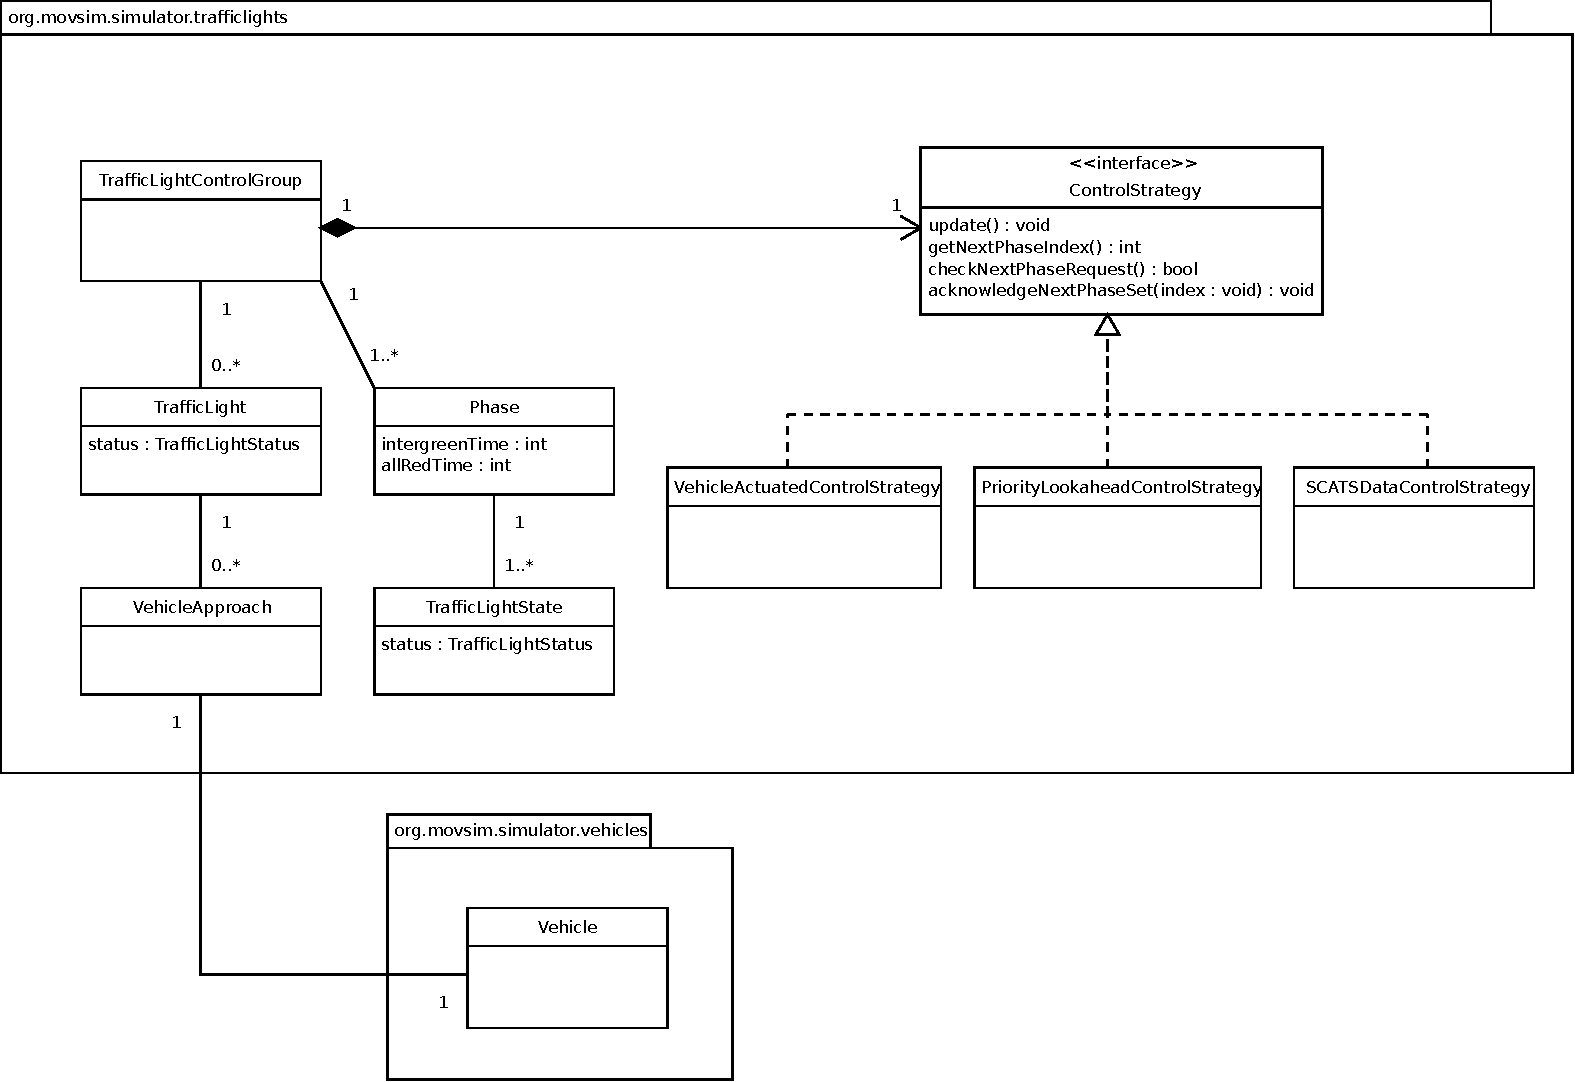
\includegraphics[scale=0.60]{controller_class_diagram.pdf}
	\caption{ A UML class diagram showing the use of the strategy pattern between the TrafficLightControlGroup and ControlStrategy types. ControlStrategy is an interface defining methods required by the TrafficLightControlGroup to change the phase of a set of traffic lights. Three strategies implementing the ControlStrategy interface are shown. Each concrete strategy implementation has a different internal set of conditions to trigger phase changes. }
\label{controllerclassdiagram}
\end{figure}

\section{Simulation of Approach Communication}

In a simulated environment, it is typically possible to access the properties of any object at any time regardless of physical laws or constraints. In order to ensure that the simulation environment used to evaluate the PBTC control system was representative of a realistic road network environment, efforts were made to ensure that the simulated communication between approaching vehicles and a traffic controller were representative of the challenges of a real-world communications network. 

Some of the primary challenges facing ad-hoc wireless communication between a traffic controller and an approaching vehicle include broadcasting and interception of the correct messages and identification of traffic controllers. Design of the network architecture required for such a system is an effort beyond the scope of this project and consideration of communication requirements was limited to ensuring reasonable lag between communication, determining what information is required for a traffic controller to estimate cost parameters, and handling repeated broadcasts from individual vehicles while approaching or waiting at an intersection.

Extending the Movsim simulation, vehicles can broadcast their state to a known traffic controller, once they are within the 150 metre communications boundary, on approach of an intersection. Each traffic controller maintains a list of broadcasts they have received as a map and each new broadcast replaces any existing broadcast from each unique vehicle. An individual broadcast contains properties required by a controller in order to calculate operational stopping cost and delay cost estimated for each individual vehicle, specifically vehicle weight, speed, acceleration, urgency, number of passengers, and distance to the intersection stop-line. 

In a simulated environment, vehicle properties can be broadcast instantly, without network costs or delay; however, in reality network topology and bandwidth limitations are factors that reduce the availability of broadcasts. To introduce allowance for imperfect network communication into the simulator, a two-second delay is imposed on each broadcast from an individual vehicle. This is not designed to be an accurate representation of network imperfections, but does reflect consideration of these factors.
 
% describe alternatives - requiring vehicles to calculate their own costs -> difficult to implement successfully, prone to hacking, difficult to update etc. etc.
An alternative to communicating physical properties of each individual vehicle to the controller is to calculate delay and stopping costs is to have these costs calculated and broadcast by the vehicle itself. This method has the advantage of reducing the amount of calculations that are required to be made by a traffic controller, however this distributed computation is more difficult to implement successfully and there are no guarantees that all vehicles will implement the same cost calculations. This method is also difficult to update if changes to the cost calculations were desired after installation.

\section{Implementation of the PBTC System}

% is this shit necessary?
The PBTC control system was implemented as a concrete ControlStrategy implementation within the Movsim project as per the algorithm and component design described in Section ~\ref{sec:PBTCDesign}.

The strategy implementation of the PBTC Control Algorithm consists of two primary phases of operation. Firstly, the implementation maintains a map of all broadcast communication packet from all vehicles approaching the intersection and dynamically calculates the sum of the individual estimated delay and operational stopping costs for all of the vehicles on each approaching link of the intersection.

The current phase will operate continuously until the calculated cost of delay on all stopped approaches exceeds than the cost of stopping green approaches, at which point the next phase is allocated and the controller enters the phase change sequence. At this point, the controller is committed to changing phases and the lookahead optimisation method is employed to determine whether the phase should change now, or some point in the future, based on the current state of vehicle statistics in the controller memory. 

% is this necessary?
\subsection{Lookahead Optimisation}

Once a PBTC controller has entered the phase change sequence, lookahead optimisation for a locally minimal cost of changing phases is found by constructing a lookahead table, forming a search space for the solution. The lookahead table includes an estimate of the  per second instantaneous change costs for all vehicles known to the PBTC controller at the time the phase change sequence was entered. 

For each second up to the defined size of the lookahead table, $K$, the PBTC control strategy implementation estimates the cost of changing phases by finding the sum of the cost of stopping, and the cost of delay at least equal to the minimum duration of the next phase in the controller sequence for every individual vehicle approaching a green signal, and the sum of the cost of stopping and cost of delay for the duration of the current lookahead for any vehicles approaching or queued at a red signal. 

The result of constructing a lookahead table is a small search space that can be efficiently queried to find the minimum estimated cost of changing phases. The lookahead time associated with the minimum cost is allocated to the extended green time for the current cycle and will delay the phase change until this time has passed.

\subsection{Vehicle Clearance Estimation}

To estimate the delay and operational stopping costs during construction of a lookahead table, a priority based traffic controller inspects the trajectory of each known vehicle based on their most recently broadcast update. In order to estimate the cost of a potential future phase change for each vehicle, the PBTC system must first determine how each individual vehicle will be affected by the phase change. For example, if a PBTC controller is considering a phase change for an intersection 5 seconds from the present time, and a vehicle is approaching at 10m/s at a distance of 30 metres, the vehicle will have passed over the intersection stop line within 3 seconds therefore will not be affected by the phase change. 

An accurate model to determine whether an individual vehicle will pass through, or "clear", an intersection within a given time frame is typically not based solely on the properties of the individual vehicle only. For example, in a free-flowing traffic situation, the distance traveled by a vehicle in a fixed time frame can be estimated using the vehicles speed and acceleration only. However, in congested traffic involving vehicle queues, whether or not a given vehicle, $v$ in the queue will clear an intersection within $t$ seconds is dependant on the speed and acceleration profiles of vehicles in front of $v$, and as a result is significantly based on driver behaviours and instantaneous traffic conditions.

Due to the difficulty of developing and implementing such a model of estimated clearances for simulation and evaluation of the PBTC system, empirical measurement of clearance times and distances within the Movsim simulator using typical driver behaviours was conducted. An experiment was conducted using the Movsim simulator to estimate the worst-case conditions of congested traffic and identify the maximum distance a vehicle could be from a traffic light to clear within a fixed range of seconds. Measurement results were used to create a map of key-value pairs consisting of the time in seconds, and the maximum distance from a traffic light a vehicle could expect to clear the intersection within the time frame.  

\section{Implementation of a SCATS Representation}

% can use the SCATS data to determine arrivals and signal settings each cycle
The SCATS implementation developed during this project was designed to recreate a representation of real-world SCATS behaviour using an available log file of vehicle arrivals and allocated phase times at different intersections in Wellington City. The SCATS log file format is shown in Appendix A, log files for intersections in Wellington City were provided for a 12 hour period of a typical day by the Wellington City Council.

Each log file consists of an ordered sequence of data blocks for a single cycle of operation for a given traffic light controller, sent to SCATS by the controller at the end of each cycle. The cycle block contains state information required by SCATS to calculate the phase timings for the next cycle, including number of vehicle detector actuations per approach, i.e. the number of vehicles that entered the intersection on each approach; and the order and time of each of the phase splits run by the controller during that cycle. 

% class diagram of scats shit here

\subsection{Vehicle Arrivals}

%The number of vehicles arriving or waiting at an intersection, also referred to as the saturation or flow rate of an intersection, is an independent variable determined by the number of vehicles on the road, criticality of an intersection to a road network. In practice, variation average flow rates for an intersection is low as commuter patterns are relatively static. The saturation of an intersection has a significant relationship with the average delay time experienced by vehicles passing through the intersection.
% fuck am i saying here?

When comparing the performance of multiple traffic control strategies, the number of vehicles input into the system should remain constant between each experiment. To account for this in the evaluation of the PBTC control system, the SCATS log files are used to determine vehicle arrivals as well as phase times for the SCATS control system. The SCATS log files can provide the exact number of vehicle actuations at each stop line inductive loop detector, for each cycle contained within an intersection log file. 

As SCATS detectors are placed on the stop line of an intersection, it is assumed that the number of vehicle actuations at each detector is approximately equal to the number of vehicles that passed through the intersection during a given green phase and for the purposes of generating vehicle arrival times, the number of vehicles that pass through an intersection during a particular phase is determined to be approximately equivalent to the number of vehicles that arrived on that approach over the entire cycle. 

This assumption is based on the fact that it is likely some vehicles will be forced to queue at a traffic light during a red phase before passing through an intersection on the next green phase. For example, for 30 vehicles to pass through an intersection during a 60 second green phase, either all of the vehicles arrived at the beginning of the green phase and were not forced to queue, or at least a number of vehicles, $v$, arrived before the begging of the green phase and formed a queue. For vehicles that arrived before the beginning of the green phase, they either arrived during a red phase and stopped at the light, or were the remainder of a queue that failed to clear in the previous green phase and had to wait after the light signal changed to red. 

By using the cycle duration as a range for estimating the exact arrival time of a given vehicle approaching an intersection, it is possible to introduce a probability function that allows for a proportion of vehicles to arrive early during a red phase, and the remainder to arrive on time during the green phase of a particular traffic light. As no other information related to the time of vehicle arrivals is available, arrival events are implemented using a Poisson arrival process. 

Given that the number of vehicle arrivals are known over the duration of a cycle, a Poisson probability function can be used to generate the time between arrivals. During simulation, the Poisson process is used to generate an estimated time to the next arrival after each simulated arrival has taken place. This model is general purpose and an improvement over the linear arrivals model that was previously implemented in Movsim. The Poisson arrivals implementation has been submitted back to the original Movsim repository as a configurable option to benefit other research investigating traffic dynamics with Movsim. 

The assumptions made here provide a reasonable estimate of the arrival time of vehicles to each queue at an intersection, as it is not possible to know the exact time of arrival and waiting time for each vehicle using only SCATS log files. The consequence of these assumptions is that generated arrival times may not be representative of the arrival times that occurred during the real-world scenario that the SCATS log files reflect, although on average it is expected the simulated arrival times will be close approximations of real-world arrivals. 

\subsection{Phase Timing}

% this section is probably shit

To create a simulation capable of emulating a real-world SCATS implementation, a traffic control strategy class was created to determine phase allocations based off the values parsed from the SCATS log files at each cycle. The SCATSDataControlStrategy is an implementation of the ControlStrategy interface designed to create a representation of SCATS behaviour.

The SCATSDataControlStrategy dynamically operates the measured phase durations contained within a SCATS log file by requesting new data from the SCATSDataParser each cycle. The SCATSDataParser is a singleton class which waits for a prompt for data from a SCATSDataControlStrategy or TrafficSource instance. The parser reads a cycle block from the log file and returns a list of phases and their durations to the SCATSDataControlStrategy, and updates each TrafficSource with a new arrival flow rate based on the phase times and vehicle arrivals measured in current cycle being read from the SCATS log. The SCATSDataControlStrategy allocates phases in order based on the list returned from the data parser and continues until the list is empty, at which point it requests another cycle and so forth.

The SCATSDataParser class is designed to respond to requests for data as it does not implement its own update method so does not have a measure of simulation time elapsed. This method ensures that a new cycle is only read from the log after the previous cycle has ended. One disadvantage of this method is that individual timers kept by each TrafficSource are not synchronised so after the cycle duration has expired, each individual TrafficSources will request the data parser to read a new cycle. Multiple cycle reads are avoided by reseting each TrafficSource after the first one has called for an update.























